\documentclass{beamer}
\usetheme{Madrid}
\usepackage{policyengine}
\usepackage{graphicx}
\usepackage{booktabs}

\title{Enhancing the CPS with Administrative Tax Data}
\subtitle{Machine Learning Meets Microsimulation}
\author[Woodruff \& Ghenis]{Nikhil Woodruff \& Max Ghenis}
\institute{PolicyEngine}
\date{National Tax Association Annual Conference\\November 14, 2024}

\begin{document}

\begin{frame}
    \titlepage
\end{frame}

\begin{frame}{Current Microsimulation Data: A Trade-off}
    \begin{itemize}
        \item Current Population Survey March Supplement (CPS)
        \begin{itemize}
            \item Rich demographics and program participation
            \item Underreports income, especially at top
            \item Limited tax information
        \end{itemize}
        \pause
        \item IRS Public Use File (PUF)
        \begin{itemize}
            \item Accurate administrative tax data
            \item No demographics or state ID
            \item Restricted access
        \end{itemize}
    \end{itemize}
\end{frame}

\begin{frame}{Data Quality: Why Accuracy and Access Matter}
    \begin{itemize}
        \item More Accurate Policy Analysis
        \begin{itemize}
            \item Taxes and benefits jointly affect household incentives
            \item Need accurate data on both to model behavior
            \item Many researchers lack access to key datasets
        \end{itemize}
        \pause
        \item Better Understanding of Economic Reality
        \begin{itemize}
            \item CPS misses top incomes
            \item PUF can't show demographic patterns
            \item Both limit inequality measurement
        \end{itemize}
    \end{itemize}
\end{frame}

\begin{frame}{Our Solution: An Open Enhanced CPS}
    \begin{itemize}
        \item Machine learning to combine strengths of CPS and PUF:
        \begin{itemize}
            \item Learn tax patterns from PUF
            \item Preserve CPS demographics and program data
            \item Optimize weights to match 570 administrative targets
        \end{itemize}
        \pause
        \item Result: First open dataset with:
        \begin{itemize}
            \item Administrative-quality tax data
            \item Rich demographics and program participation
            \item Transparent, reproducible methodology
        \end{itemize}
    \end{itemize}
\end{frame}

\begin{frame}{Two-Stage Approach: ML Imputation + Weight Optimization}
    \begin{figure}
        \centering
        \includegraphics[width=\textwidth]{../../paper/figures/data_flow.png}
        \caption{Overview of dataset enhancement process}
    \end{figure}
\end{frame}

\begin{frame}{Quantile Regression Forests: Beyond Statistical Matching}
    \begin{itemize}
        \item Standard approach: statistical matching or regression
        \item We use Quantile Regression Forests (QRF) for:
        \begin{itemize}
            \item Imputing tax variables from PUF
            \item Predicting housing costs from ACS
            \item Estimating prior year earnings
        \end{itemize}
        \item Benefits of QRF approach:
        \begin{itemize}
            \item Captures full conditional distributions
            \item Handles non-linear relationships
            \item Preserves correlations between variables
        \end{itemize}
    \end{itemize}
\end{frame}

\begin{frame}{QRF Outperforms Traditional Imputation Methods}
    \begin{figure}
        \centering
        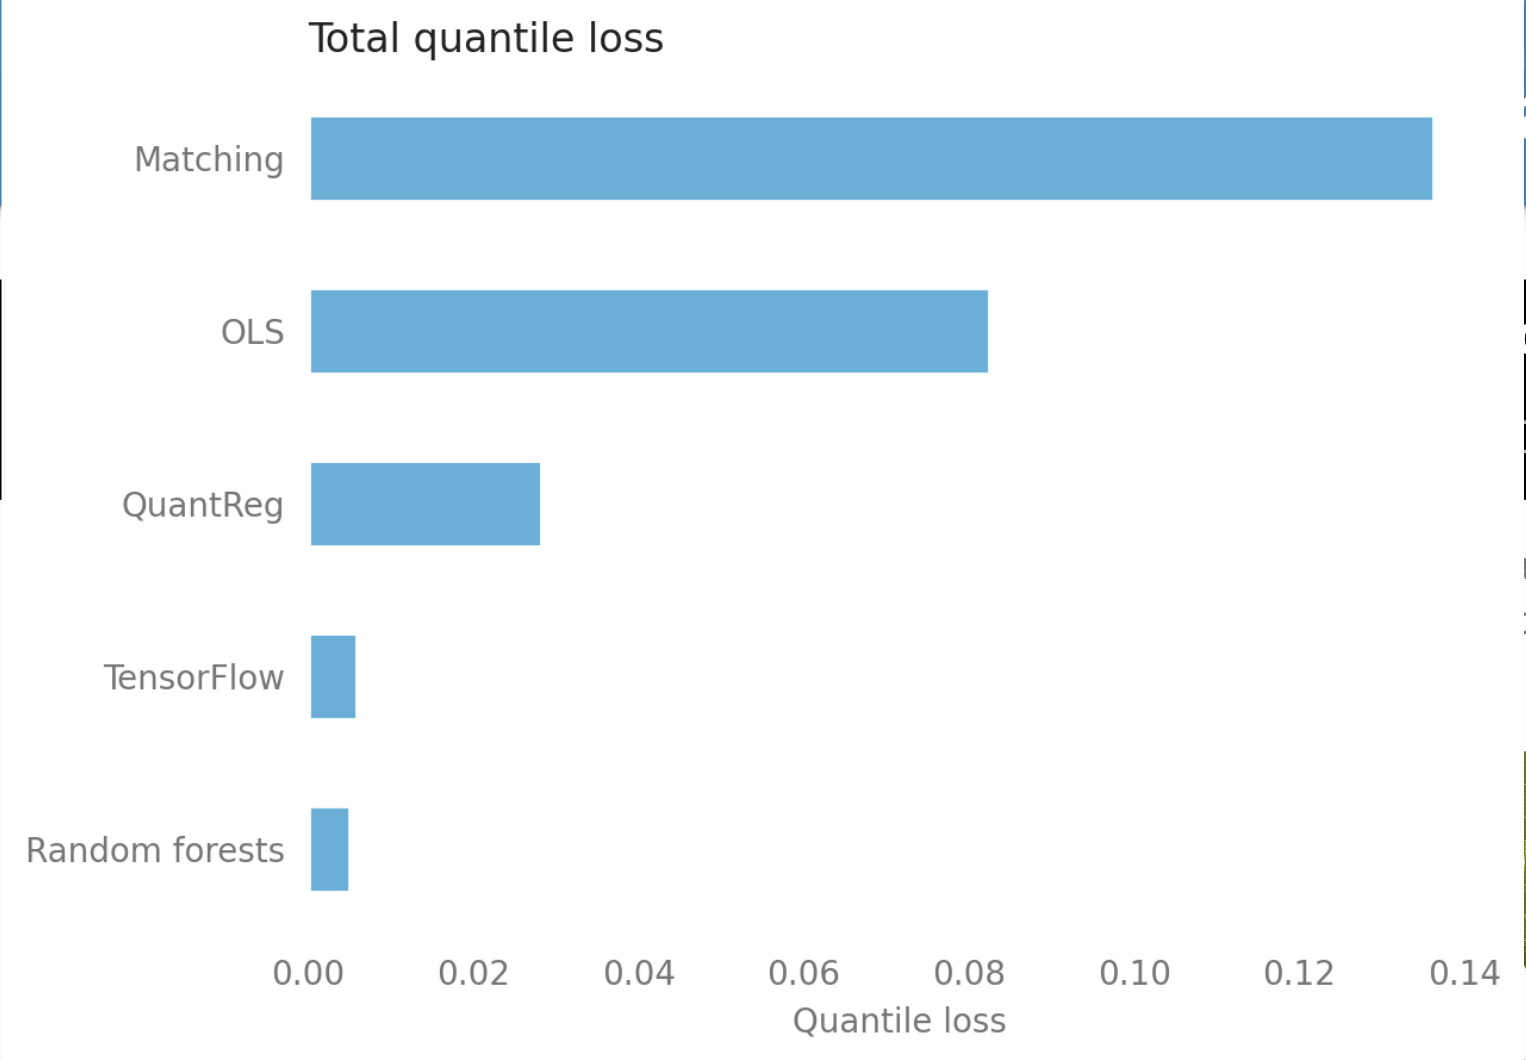
\includegraphics[width=0.9\textwidth, height=0.7\textheight, keepaspectratio]{../../paper/figures/quantile_loss.png}
        \caption{Average quantile loss by method, predicting net worth from covariates in SCF}
    \end{figure}
\end{frame}

\begin{frame}{Calibration: 570 Simultaneous Targets}
    \begin{itemize}
        \item Standard approach: constrained optimization
        \item We use dropout-regularized gradient descent
        \item Optimizes against 570 targets:
        \begin{itemize}
            \item IRS Statistics of Income by income bins
            \item Program participation totals
            \item Single-year age population counts
        \end{itemize}
        \item Mathematics:
        \[ L(w) = \text{mean}\left(\left(\frac{w^T M + 1}{t + 1} - 1\right)^2\right) \]
        where $w$ are weights, $M$ is characteristics, $t$ are targets
    \end{itemize}
\end{frame}

\begin{frame}{Validation I: Selected Target Comparisons}
    \begin{table}
        \small
        \centering
        \begin{table}[h]
    \centering
    \caption{Examples of calibration targets by source}
    \label{tab:target_examples}
    \begin{tabular}{lll}
    \toprule
    Source & Example Targets & Count \\
    \midrule
    IRS SOI & AGI by bracket, employment income, capital gains & 5,300+ \\
    Census & Population by age, state populations & 150+ \\
    CBO & SNAP benefits, Social Security, income tax & 5 \\
    JCT & SALT deduction (\$21.2B), charitable (\$65.3B) & 4 \\
    Healthcare & Medicare Part B premiums by age group & 40+ \\
    \bottomrule
    \end{tabular}
\end{table}

    \end{table}
    \begin{itemize}
        \item ECPS is best on qualified dividends and infant population
        \item PUF better on returns AGI 100-200k
        \item 567 other targets!
    \end{itemize}
\end{frame}

\begin{frame}{Validation II: ECPS Outperforms Both Source Datasets}
    \begin{figure}
        \centering
        \includegraphics[width=\textwidth]{../../paper/figures/ecps_vs_cps_puf.png}
        \caption{Error change from ECPS to better of CPS and PUF}
    \end{figure}
    \begin{itemize}
        \item ECPS outperforms CPS on 63\% of targets
        \item ECPS outperforms PUF on 71\% of targets
    \end{itemize}
\end{frame}

\begin{frame}{Validation III: Matching PUF Income Distribution}
    \begin{table}
        \centering
        \begin{table}[h]
    \centering
    \caption{Key tax unit-level distributional metrics}
    \label{tab:tax_unit_metrics}
    \begin{tabular}{lrrr}
    \toprule
    Metric & CPS & Enhanced CPS & PUF \\
    \midrule
    Gini coefficient & 0.495 & 0.572 & 0.570 \\
    Top 10\% share & 0.361 & 0.425 & 0.410 \\
    Top 1\% share & 0.085 & 0.154 & 0.150 \\
    \bottomrule
    \end{tabular}
\end{table}

    \end{table}
    \begin{itemize}
        \item CPS inequality measures 12-45\% lower than PUF
        \item ECPS inequality within 4\% of PUF
        \item Unlike PUF, ECPS includes nonfilers
        \item Inequality measured as income after taxes and transfers
    \end{itemize}
\end{frame}

\begin{frame}{Application: Top Tax Rate Reform Analysis}
    \begin{itemize}
        \item Example: Biden's proposed top rate increase
        \item Would raise rate from 37\% to 39.6\% above \$400k
    \end{itemize}
    \begin{table}
        \centering
        \begin{table}[h]
    \centering
    \caption{Revenue projections from top rate increase (37\% to 39.6\%)}
    \label{tab:top_rate_reform}
    \begin{tabular}{llll}
    \toprule
    Dataset & Revenue Impact (\$B) & Affected Tax Units (M) & Avg Tax Increase (\$) \\
    \midrule
    CPS & [TBC] & [TBC] & [TBC] \\
    Enhanced CPS & [TBC] & [TBC] & [TBC] \\
    PUF & [TBC] & [TBC] & [TBC] \\
    \bottomrule
    \end{tabular}
\end{table}

    \end{table}
    \begin{itemize}
        \item Can analyze by demographics, geography, income
        \item Interactive results at policyengine.org
    \end{itemize}
\end{frame}

\begin{frame}{Unique Capability: Direct Demographic Analysis}
    \begin{itemize}
        \item Direct race/ethnicity analysis without imputation
        \item Other models use complex methods:
        \begin{itemize}
            \item CBO: Statistical matching with Census data
            \item Tax Policy Center: Multiple copies with reweighting
            \item ITEP: Probability assignment based on characteristics
        \end{itemize}
        \item Our approach:
        \begin{itemize}
            \item Uses observed demographics from CPS
            \item Individual-level rather than tax unit only
            \item Enables analysis of intersectional effects
            \item Extends to disability, education, etc.
        \end{itemize}
    \end{itemize}
\end{frame}

\begin{frame}{Implementation: Open Code and Growing Usage}
    \begin{itemize}
        \item Full codebase on GitHub
        \item Automatic validation dashboard
        \item Python package for programmatic access
        \item Web interface at policyengine.org
        \item Growing research applications:
        \begin{itemize}
            \item Academic studies
            \item Think tank analysis
            \item Government agency use
            \item Community contributions
        \end{itemize}
    \end{itemize}
\end{frame}

\begin{frame}{PolicyEngine: Interactive Policy Analysis}
    \begin{figure}
        \centering
        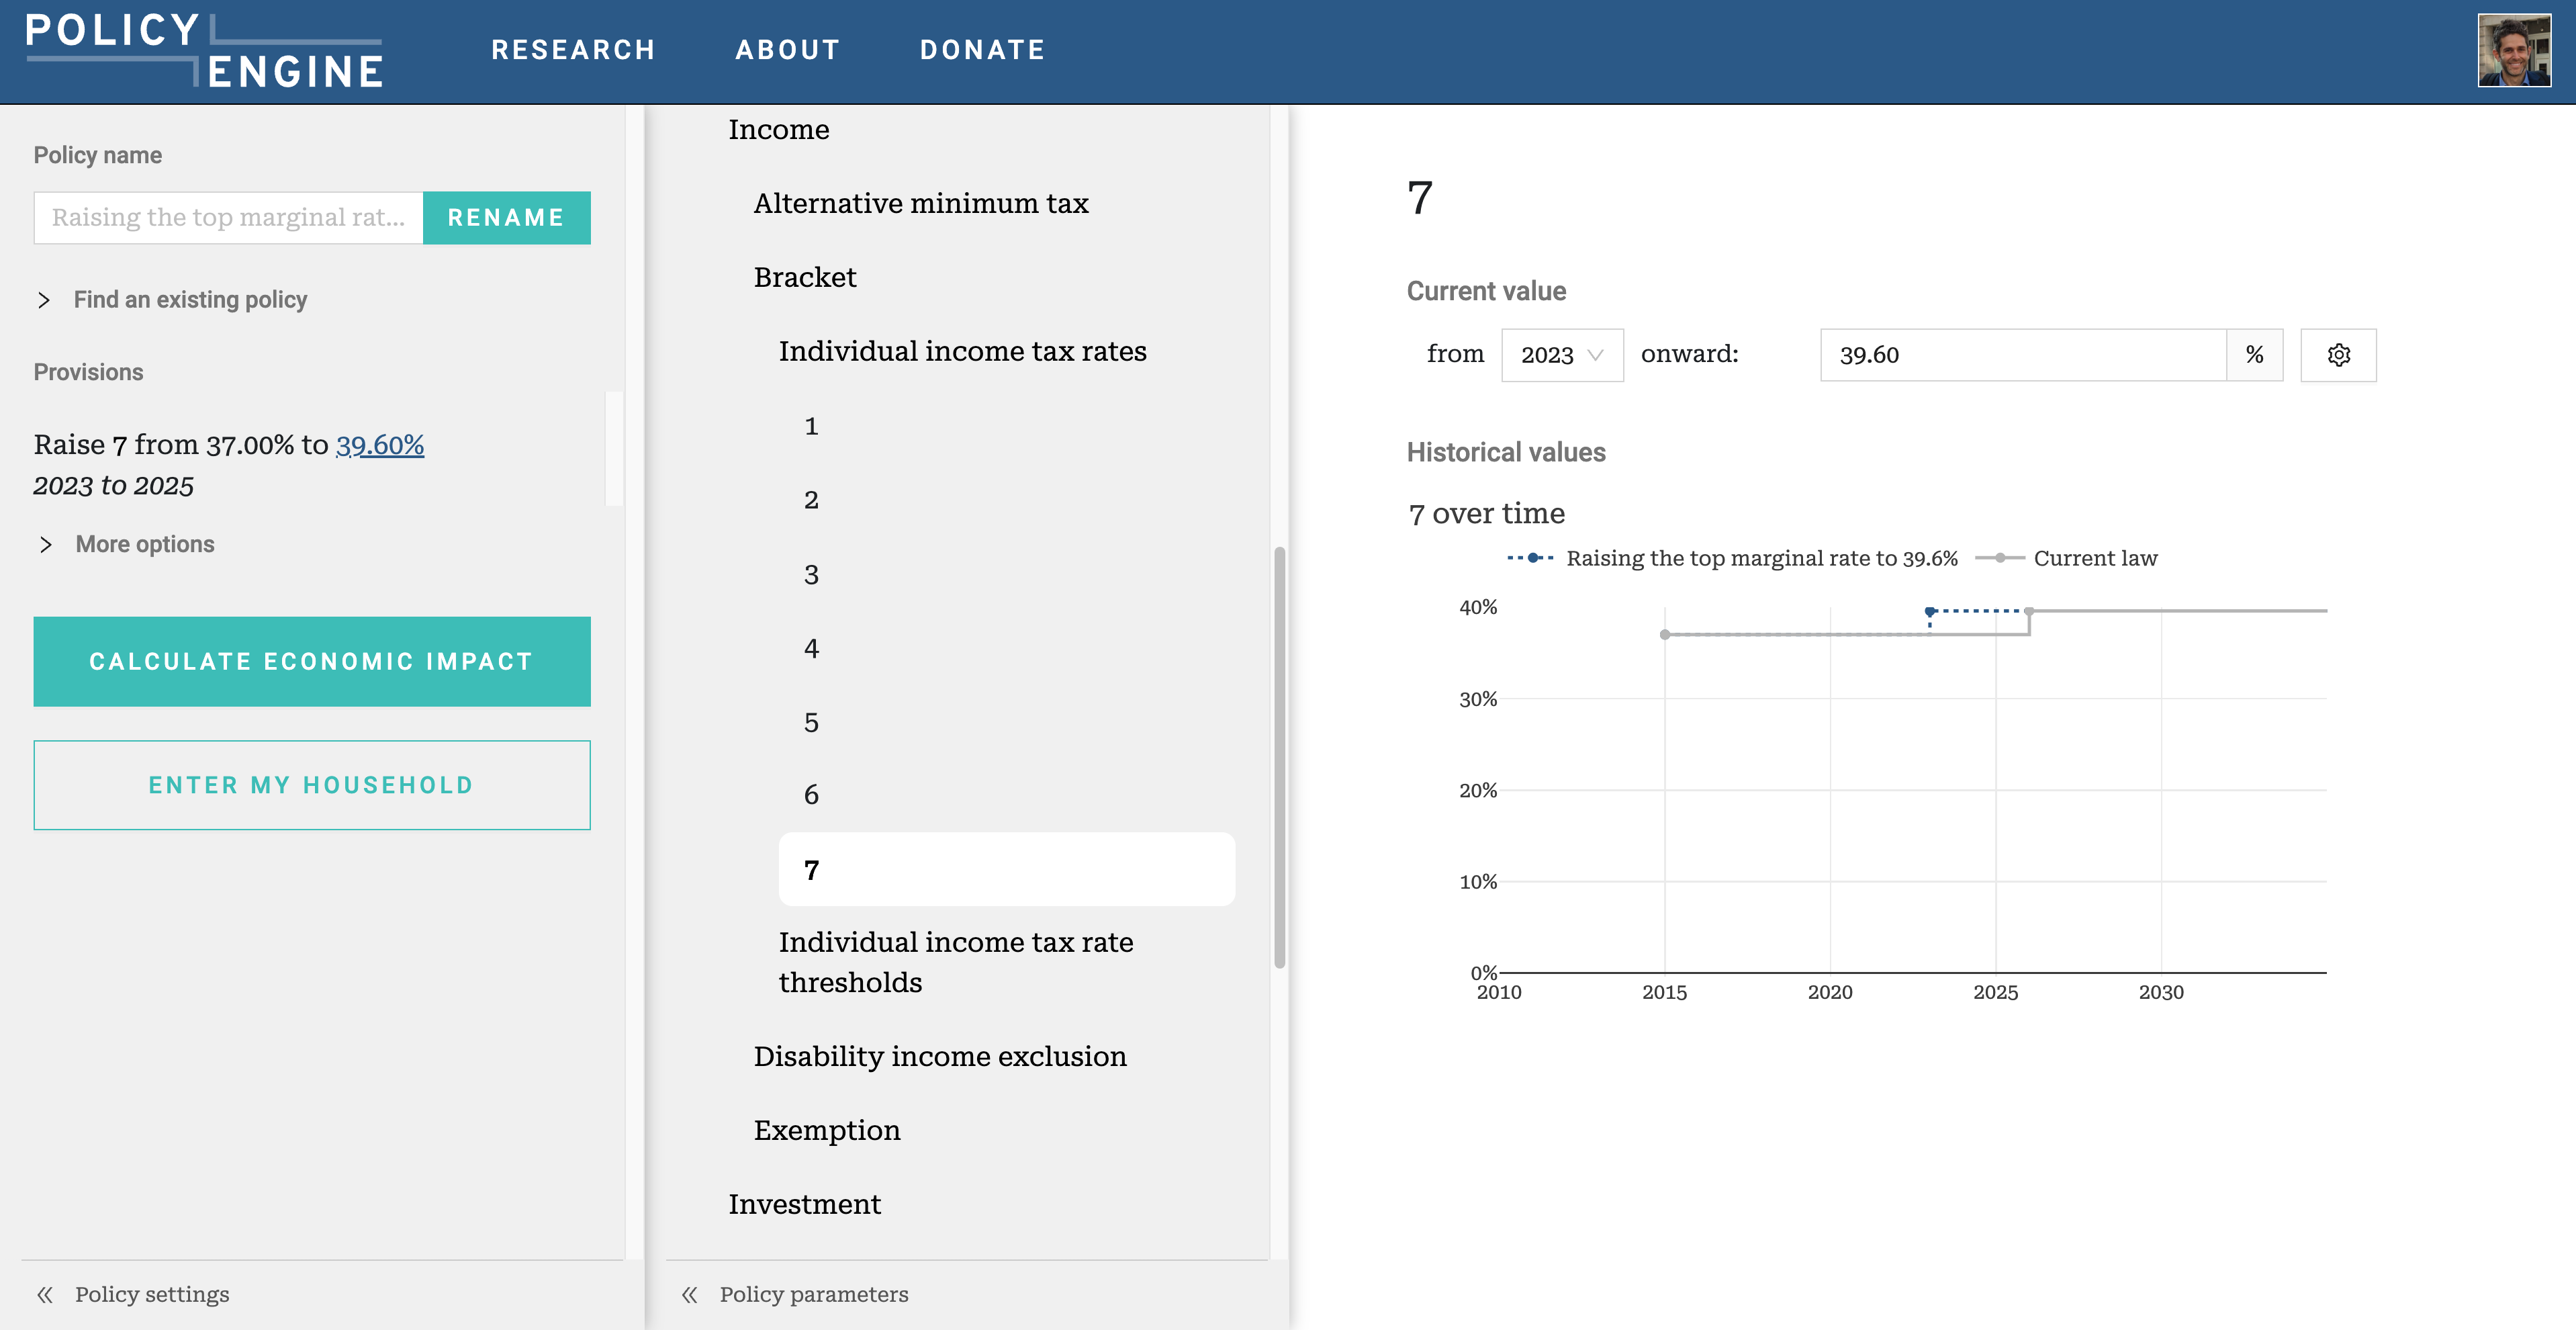
\includegraphics[width=\textwidth]{../../paper/figures/policyengine_policy.png}
        \caption{PolicyEngine's policy editor interface}
    \end{figure}
\end{frame}

\begin{frame}{PolicyEngine: Interactive Policy Analysis}
    \begin{figure}
        \centering
        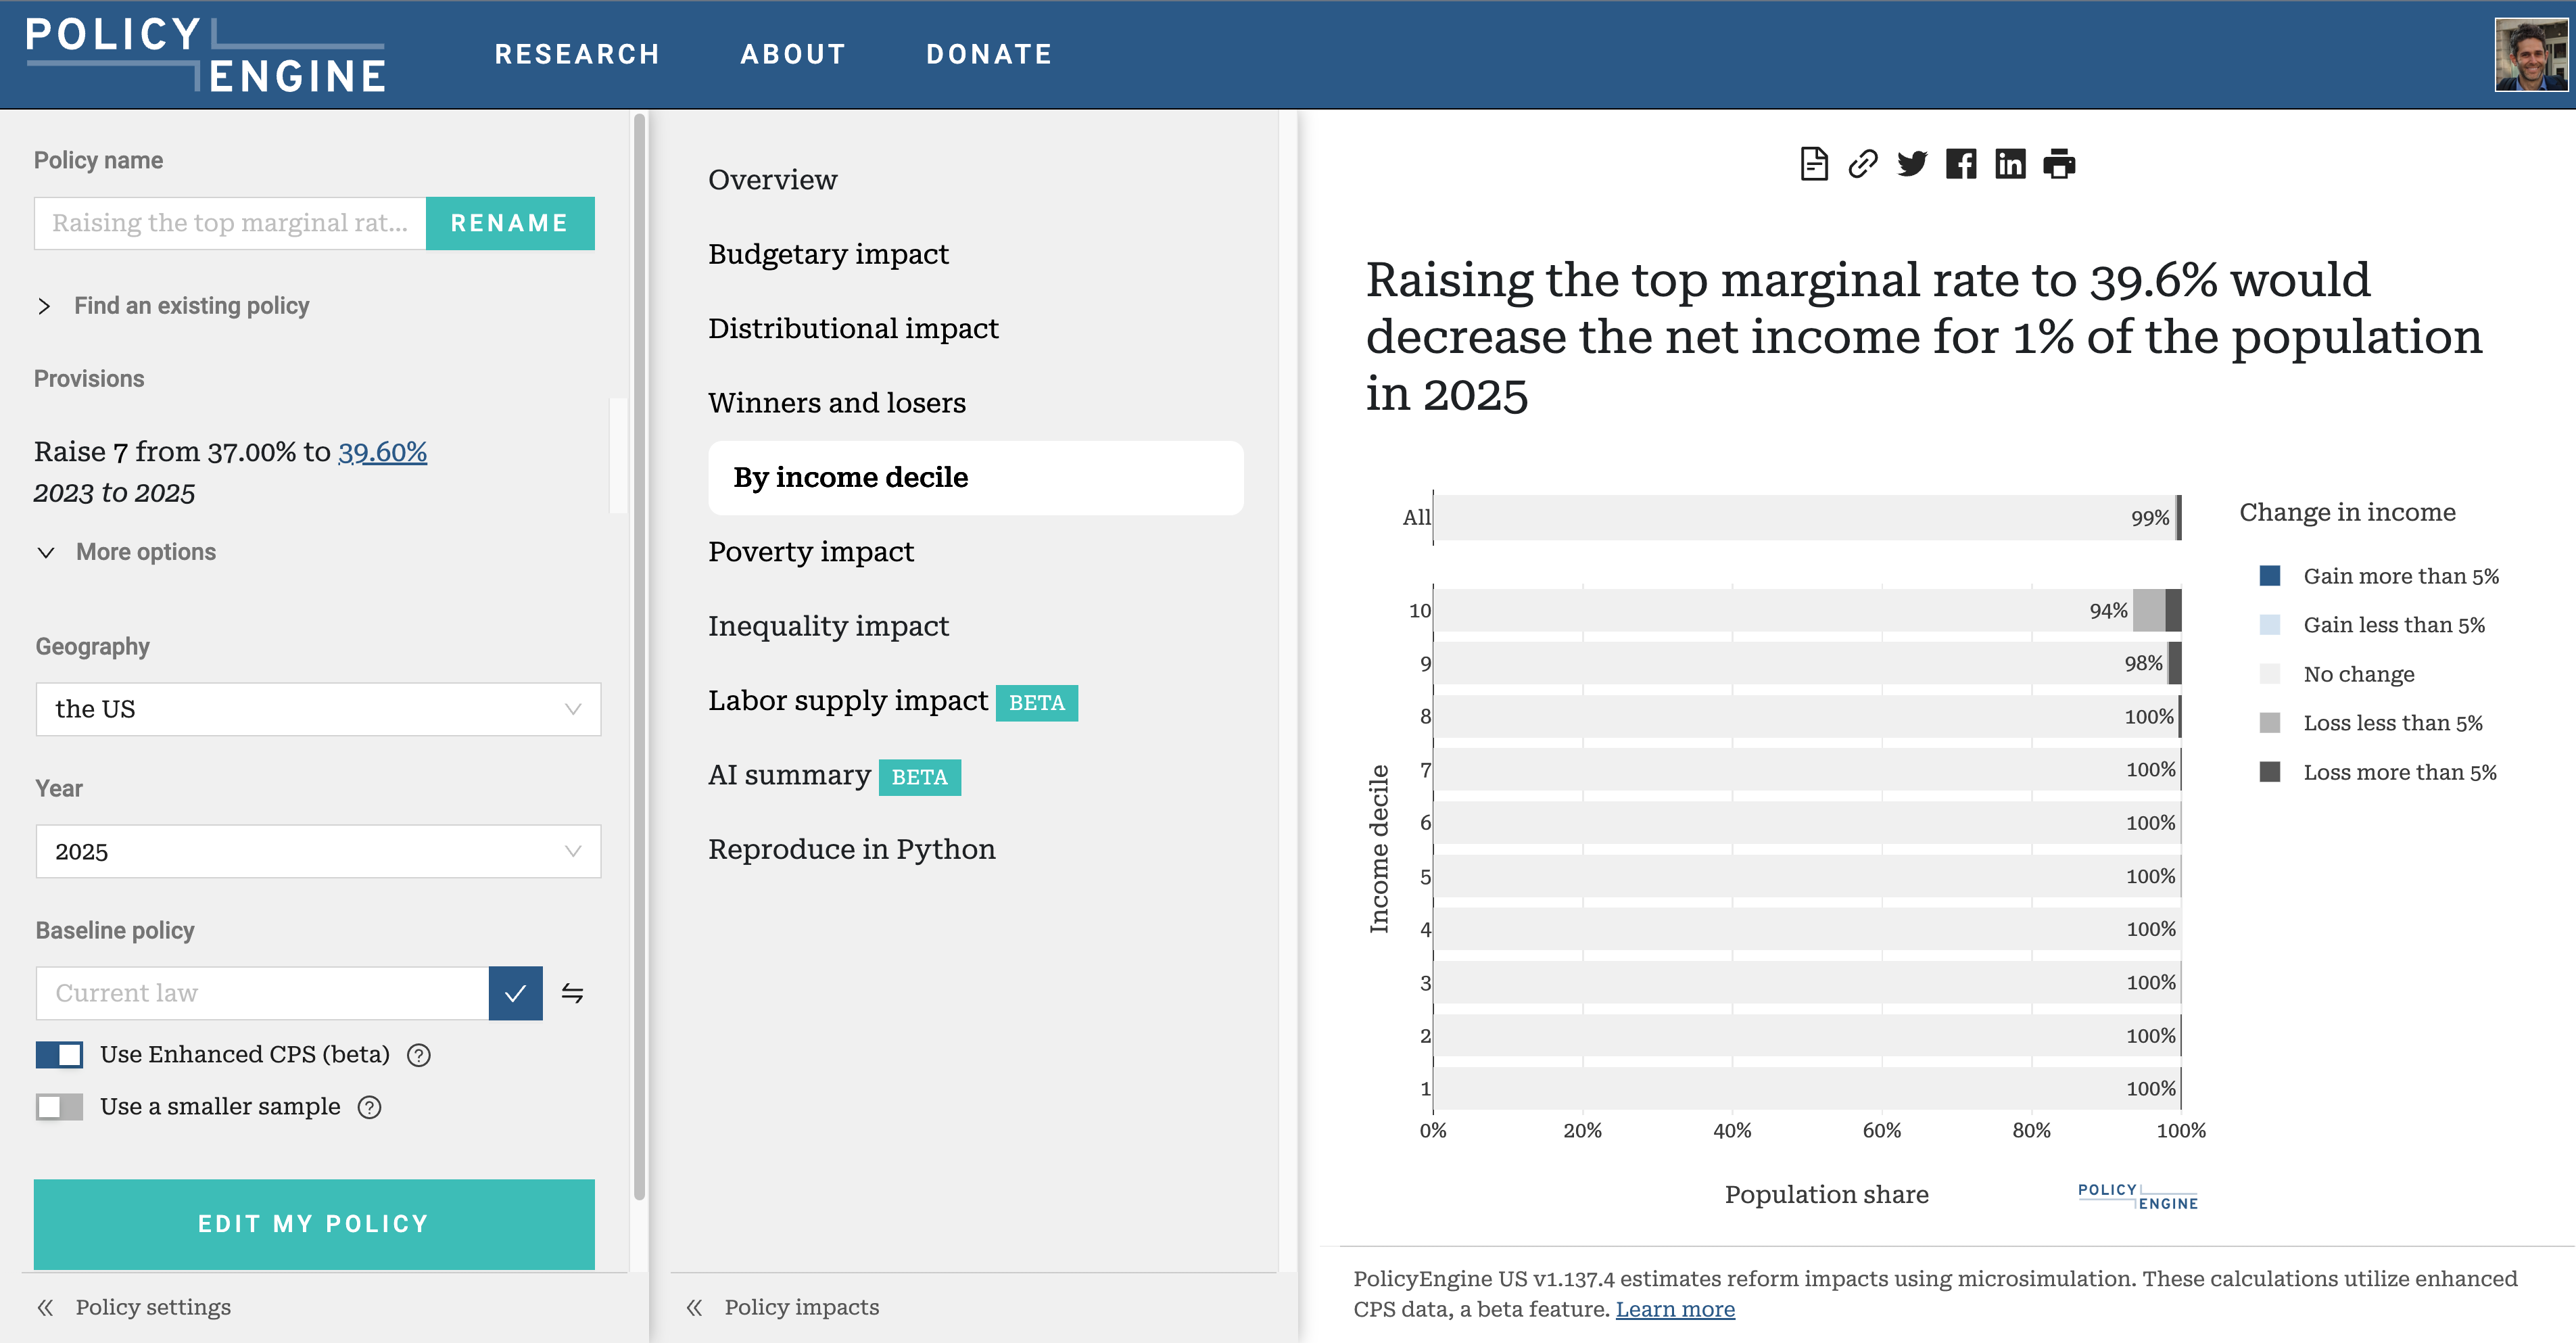
\includegraphics[width=\textwidth]{../../paper/figures/policyengine_results.png}
        \caption{PolicyEngine's policy impact interface}
    \end{figure}
\end{frame}

\begin{frame}{Future Work: Geographic Detail and Validation}
    \begin{itemize}
        \item Geographic extensions:
        \begin{itemize}
            \item Congressional district weights
            \item State-specific calibration
            \item County-level synthetic data
        \end{itemize}
        \item Prediction-oriented validation:
        \begin{itemize}
            \item Compare to tax expenditure reports
            \item Backtest
            \item Benchmark ML architectures
        \end{itemize}
        \item International applications (UK version live)
    \end{itemize}
\end{frame}

\begin{frame}{Thank You}
    \begin{itemize}
        \item Paper: github.com/PolicyEngine/policyengine-us-data/paper
        \item Code: github.com/PolicyEngine/policyengine-us-data
        \item Web app: policyengine.org
        \item Contact: max@policyengine.org
    \end{itemize}
\end{frame}

\end{document}
